\chapter{Types}
\label{types}

\lettrine[nindent=0.1em]{G}{o! is a statically checked} strongly typed language. Strong typing means that every variable and every expression has a single type associated with it, and that the uses of these expressions are consistent with expectations. Static type checking means simply that types are checked at compile-time rather than at run-time.

Strong static typing greatly enhances confidence in the correctness of programs -- as a large number of programmer errors can be caught simply by virtue of the wrong kind of value being passed into functions (or other rule programs). In addition, strong typing also enhances the potential for automatic tools to support the \go programmer. For example, using type information available in a \go program, one can automatically generate `glue' code for interfacing \go applications to other programming languages such as Java and link to Internet standard message specifications such as SOAP.\note{This is currently a potential benefit rather than one realized: at this time there are no source automation systems available for \go.} Such automation has the potential to greatly relieve the programmer's burden for integration.

However, perhaps the strongest reason for adopting a strong typing system is simply that types are a natural aspect of programming: programmers must nearly always have some idea of what kinds of values an argument or variable can take. A programming language that does not support explicit typing forces the programmer to throw away this information -- unless it is captured in comments. However, for correctness, \emph{some} form of typing is required dynamically. For example, arithmetic applies to numeric values, not lists. A system that relies on dynamic typing must recover the programmer's intention at run-time; a waste given that those intentions were always present and are probably written as comments!

\go's type system is founded on three key concepts. The \firstterm{type expression}{A term that \emph{denotes} a type. A simple type expression would be something like the symbol \q{char} -- which denotes the type of character expressions. A more complex example would be \q{list[char]} which denotes lists of characters -- i.e., strings} is a term that denotes a type -- normally the type of a variable or other expression.

Type expressions are related to each other by the \emph{sub-type} relation: which represents a partial ordering on type terms. The sub-type relation is indicated by the programmer explicitly declaring which type terms are sub-types of other type terms -- as part of type definition statements.

The second key concept is the \firstterm{type interface}{An interface is associated with a type that defines the legal operations on values of that type. More specifically, the interface defines the expressions possible on the right hand side of a `dot' expression.}. A type interface defines the interface to a labeled theory -- specifically, it defines the kinds of `dot' references that are supported by a given type of value. All named types may support an interface and many system types also support an interface. If the type term defines what kind of value an expression has, the type interface defines to a large extent what you can do with the value.

Finally, \firstterm{type inference}{Type inference is the process by which a type expression can be \emph{automatically} assigned to an identifier or expression \emph{without} requiring that the type of the identifier be explicitly declared.} is used to reduce the burden of annotating a program with type expressions. Programs and top-level names are \emph{declared}, type inference is used to verify that program rules \emph{conform} to the declared type. Type inference allows the types of rule argument variables and pattern variables to be automatically inferred; a signifant saving in a rule-oriented language.

In this chapter we look in greater detail at the kinds of type terms that you may come across and also cover issues such as defining your own types and interfaces.

\begin{aside}
There is more than one way of introducing types into a logic language; our approach is intended to take advantage of modern type checking technology; in particular the Hindley/Milner \cite{hindley:69}, \cite{milner:78} type inference algorithms.

Another potential type system is to use so-called distinguished unary predicates. Unfortunately, this approach is less amenable to static type checking than the \emph{abstract interpretation} approach adopted here.
\end{aside}

\section{Type terms}
\label{type:term}
\index{type terms}

A type expression is a kind of logical term whose interpretation is fixed by the \go language. For example, the symbol \q{char} is the term that is used to denote the character type. The term \q{list[char]} is a slightly more complex (compound) term that denotes the type `list of \q{char}' -- i.e., strings. Although technically type expressions are terms, they are \emph{separated} in \go from ordinary terms: type terms are never legal values of ordinary variables, and programs cannot `manipulate' type terms.

\begin{aside}
To help distinguish type terms from regular terms we use square brackets for type constructor terms -- as opposed to round parentheses for normal terms.
\end{aside}

Every expression in a \go program is associated with a type term which is called the expression's \firstterm{type assignment}{A mapping from an expression to a type term} or \emph{type denotation}. The process of type checking is essentially that of performing the type assignment, and a type error results if we cannot assign types in a consistent way.

In addition to the type assignment, there are a number of \firstterm{type constraints}{a type constraint is a predicate that must be satisfied if the program is to be \emph{type safe}.}. Type constraints encode the rules for type safety in programs. There are two kinds of type constraints, type \emph{inequality} constraints that reflect the sub-type relationship and \emph{program} constraints that reflect the program being type checked.

Every syntactic form in the \go language has either or both a type assignment and type constraint associated with it.

\subsection{A lattice of types}
The set of type terms forms a \firstterm{type lattice}{a partial ordering with an identified \q{top} element that is bigger than all others, and a bottom element \q{void} that is smaller than all other elements.}. A lattice is simply a set with a partial ordering associated; together with a top element (\q{top} in \go's case) and a bottom element (\q{void}). A type lattice is a kind of lattice where the elements are type terms; and the partial ordering is, in fact, the \emph{sub-type} relation. 

\begin{figure}
\centerline{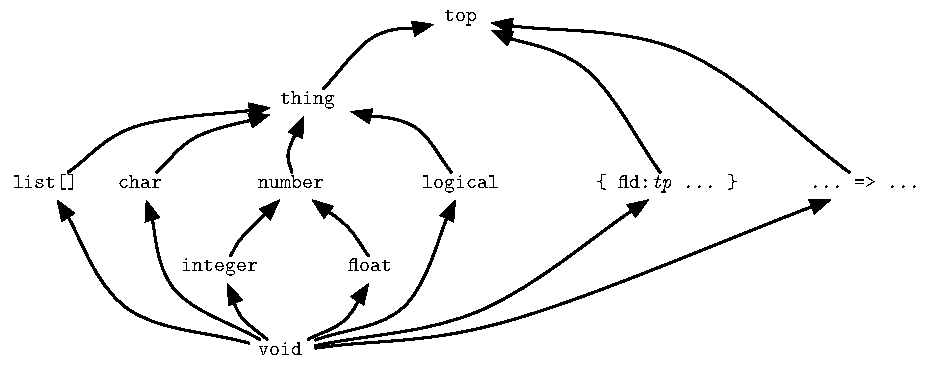
\includegraphics[width=\textwidth]{lattice}}
\caption{\label{type:lattice}Part of \go's standard type lattice}
\end{figure}

The sub-type relation encodes the relationship between types, higher in the order means more general and lower in the ordering means more specific. Thus \q{top} type is the most general type (and therefore the least is known about values of type \q{top}) and \q{void} is so specific that there are \emph{no} legal \q{void} values.

The significance of \q{top} and \q{void} is largely technical, however, a function that accepts \q{top} arguments will accept anything and a \q{void} value is acceptable for all functions. On the whole, if you see either \q{top} or \q{void} in a type expression in an error message, you are likely to be in trouble!

You will notice that \go's type lattice is wide and shallow -- that for the most part there are few significant \firstterm{chain}{A chain is a sequence of types where for each pair of types in the link \emph{T\subi} and \emph{T\sub{i+1}} it  known that \emph{T\subi} is a subtype of \emph{T\sub{i+1}}. All types are in a chain of at least three elements: \q{void}, the type itself and \q{top}.}s in the lattice. This is in the nature of type systems. However, when defining types, and inheriting types, then we do get a richer network. For example, figure~\vref{type:dynrel} shows the lattice associated with the \q{dynRule[]} type in program~\vref{meta:rules}.

This graph highlights the fact that a lattice is not necessarily a simple \firstterm{basket}{A basket type lattice is one where every chain is exactly three elements long; meaning that there is no significant subtype relationship between non-trivial type elements.} or \emph{chain}, but can have have branching elements in it. It cannot, however, have cycles -- a lattice with a cycle is not permitted.

\begin{figure}
\centerline{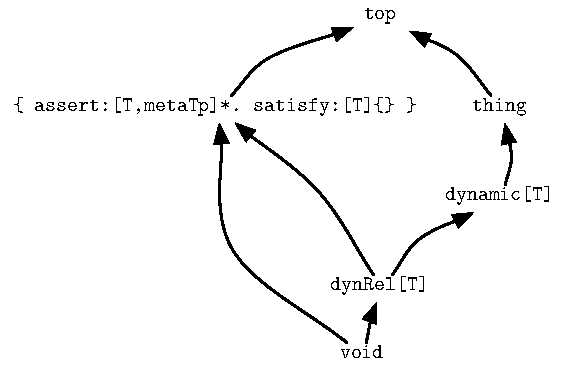
\includegraphics[width=0.75\textwidth]{dynrel}}
\caption{\label{type:dynrel}The type lattice associated with \q{dynRel[]}}
\end{figure}

There is, of course, a standard definition of the ordering of \go's types. For the most part it is fairly straightforward: everything is bigger than \q{void}, smaller than \q{top}. Every type definition statement such as:
\begin{alltt}
student \typearrow person
\end{alltt}
is actually a rule of the \q{\typearrow} relation; that defines the ordering between two type expressions.

In addition to these specific declarations, the rules that correspond to \go's standard types are built-in. Two of these rules may be of interest: the rule for function types and the rule for type interfaces.

The rule for function types is interesting because of its \emph{contra-vari\-ance}. For one function type to be less than another, the result type must be less, but the arguments must be larger.\note{Whenever we talk about one type being less than another we also allow that the types are \emph{equal}.}

The intuition behind the sub-type relation is that a smaller value than that expected should be an acceptable replacement as an argument to a function -- if a \q{student} is a \q{person}, then a \q{student} is an acceptable replacement for any function expecting a \q{person}. For a \emph{function} to be an acceptable replacement, it must accept all arguments (and perhaps more) than those expected and must return a value that is an acceptable replacement for the expected result.

The rule for \emph{type interfaces} is that any \emph{named} type is smaller than its corresponding interface. The intuition here is that naming a type somehow adds information that is not present in the interface itself: naming a \q{person} type gives more information and is stronger than merely the interface for a \q{person}. This rule is particularly important when type checking references to objects.

\subsection{Type variables}
\label{types:standard:variable}

A type variable is a variable -- ranging over type terms only -- that denotes a type. Most often, type variables are assigned implicitly and automatically by the compiler as part of the type checking process -- for example, each identifier in the program will automatically have a type variable associated with it when it is first encountered. 

All type variables have two types associated with them: an upper bound and a lower bound. A completely unconstrained type variable is still less than (or equal to) \q{top} and larger than (or equal to) \q{void}:
\begin{alltt}
void \typearrow V \typearrow top
\end{alltt}
\go's compiler will not display a variable's lower and upper bounds unless they are different from \q{void} and \q{top} respectively.

\begin{aside}
\go's compiler is based on a relatively strong assumption about these lower and upper bounds: that they always exist and that they are never themselves unbound type variables. That a variable always has an upper and lower bound is guaranteed by the \q{void} and \q{top} types. That these bounds are non-variable is an assumption that is stronger than that sanctioned by lattice theory.
\end{aside}
\begin{aside}
On the other hand, in practice, this is not as draconian as it seems. The only situation where type inference might ordinarily infer that one type variable was less than another is in typing polymorphic programs. Most such programs are recursive; a fact which tends to force type variables to be equal to each other.
\end{aside}
\begin{aside}
\go's type system, when it is asked to infer that two type variables are in the \typearrow relation, simply assumes that they must be equal. That is sufficient to eliminate all \emph{variable}\typearrow\emph{variable} chains.
\end{aside}
\begin{aside}
Pragmatically, what this means is that the sub-type relationships between types take effect only where the types are known. I.e., if a function is expecting a \q{person} value and the actual argument is known to be of \q{student} type, then the type analysis will permit it -- providing of course that it can determine that \q{student} is less than \q{person}.
\end{aside}
\begin{aside}
Besides considerably simplifying type inference, eliminating variable chains has another benefit -- of simplifying error messages. Without such a simplification error messages could easily become impossible to read.
\end{aside}


\subsection{Polymorphism and type quantification}
\index{type!polymorphism}
Although \go requires that each identifier has just one type associated with it, types and programs may be \firstterm{polymorphic}{A polymorphic type is one which is quantified. For example:\\
\q{[s]=>list[s]}\\
is a type expression that denotes a polymorphic function type. A function of this type can be applied to any kind of argument type (\q{\emph{A\sub{t}}} say), and the result of a function application will have type \q{list[\emph{A\sub{t}}]}}. 

Polymorphism means variable shape; in type theory it means variable type. In type theory there are two main kinds of polymorphism -- sub-type polymorphism and parametric polymorphism.

Sub-type polymorphism refers to a variability in the value of a variable based on sub-types: a variable of a given type can take any value of that type or of a sub-type of that type. For example, \q{float} is a sub-type of \q{number}, in which case, with sub-type polymorphism, a \q{float} value is an acceptable value for a \q{number} argument to a function. Sub-type polymorphism is often used in Object Oriented languages as it relates well to the basic sub-type relationships between classes. 

If sub-type polymorphism is a \emph{don't care} kind of polymorphism, parametric polymorphism is a \emph{don't know} form of polymorphism. A \go list, for example, may have any kind of elements -- but they must all be of the same type. For a given list expression it may not be known what the type of each element is, but it does have a unique type. 

The two forms of polymorphism are different: neither can be described in terms of the other; although either is able to accurately represent most given program situations -- with differing styles and levels of syntactic markup. 

In \go we combine both parametric and sub-type polymorphism; however, the requirement that programs and top-level names be explicitly declared means that we are never required to compute program types. This simplification makes the overall type inference process easier, and, more importantly, makes error messages significantly shorter.

Polymorphism is reflected in type terms also -- they can have type arguments. For example, the \q{char} type is the type associated with characters; and \q{list[char]} represents the type list  of \q{char}s. The list type (\q{list[\emph{type}]}) is polymorphic: it has a type argument which is the type of the elements of the list.

\paragraph{Quantified types}
\label{type:quantification}
\index{type quantification}
Associated with the concept of polymorphism is \emph{type quantification}. 
A quantified type term is one that represents infinitely many types -- a kind of type schema -- each variant gotten by substituting type expressions for occurrences of the bound type variable. A quantified type consists of a \emph{bound variable} and a type expression -- presumably mentioning the bound variable. 

The distinction between a polymorphic type and a quantified type is one of range: a type expression may have within it type variables -- signifying a lack of knowledge about the actual type. A fully quantified type also has type variables within it, but the bound variable indicates that the type is valid for any substitution of that variable.

When a polymorphic type expression is encountered in a program, the \go compiler  automatically determines the quantifiers; however we can, if we wish, write them explicitly:
\begin{alltt}
(<>):[t]-[[list[t],list[t]]=>list[t]
\end{alltt}

We can combine such quantified types with a sub-type constraint. For example, the types of the built-in arithmetic functions are polymorphic -- with a constraint that the arguments are at least \q{number}:
\begin{alltt}
(+):[t\typearrow number]-[t,t]=>t
\end{alltt}
This type declaration states that the \q{+} function is a polymorphic function that takes any kind of argument which is less than -- or equal to -- \q{number} and returns a value of the same type. In particular, of course, the \q{float} and \q{integer} types. Whichever type of argument it is given, it will return a value of the same type -- given two \q{integer}s, it will return an \q{integer} result.

The converse of type quantification is \emph{standardizing apart}. In this process a quantified type expression is \emph{refreshed} -- rewritten from a quantified from to a non-quantified form. This is done by the type inference process for each occurrence of an identifier; most importantly for function calls.

One situation where explicit quantifiers are sometimes called for is in interface descriptions. If a type is to have a polymorphic function (say) in its interface, and the bound variable is \emph{not} bound by the type itself, then the function type \emph{must} be explicitly quantified.

For example, suppose we have a type -- \q{comp} -- which has a polymorphic \q{less} predicate in its interface. We might write this as:
\begin{alltt}
comp \typearrow \{ less:[t]-[t,t]\{\} \}.
\end{alltt}
Note that \q{comp} is \emph{not} polymorphic; however it includes in its interface the polymorphic predicate \q{less}. Compare this definition with:
\begin{alltt}
cmp[t] \typearrow \{ less:[t,t]\{\} \}.
\end{alltt}
where \q{cmp} is polymorphic and \q{less}, while polymorphic is not locally quantified. The difference is the extent to which the polymorphism \emph{leaks}: a variable of type \q{comp} will allow any values to be compared using \q{less}
\begin{alltt}
\{
  p:[comp]\{\}.
  p(O) :- O.less(2,3), \ldots, O.less('a',X).
\}
\end{alltt}
this rule, while a little bizarre, is legitimate because the \q{less} predicate is locally  quantified. However, the program:
\begin{alltt}
\{
  p:[cmp[integer]]\{\}.
  p(O) :- O.less(2,3), \ldots, O.less('a',X).
\}
\end{alltt}
will raise a syntax error with the compiler -- because while \q{2} and \q{3} are \q{integer}s, \q{'a'} is a \q{symbol} which is not compatible with \q{integer}. Notice how with \q{cmp} we have to select a value for the type parameter, we don't have to with \q{comp}.

\begin{aside}
There is a special obligation incurred when declaring a program to be polymorphic. Fundamentally, generic or polymorphic programs never examine the values associated with the polymorphic type variable. In particular, they \emph{never} match a value whose type is represented by a type variable against a literal value.

So, for example, the program
\begin{alltt}
p:[t]\{\}.
p(23)
\end{alltt}
is not legal because the polymorphism assumption is violated: \q{p} is supposed to make no assumptions about the type of the first argument. The natural type of the \q{p} program is 
\begin{alltt}
p:[integer]\{\}
\end{alltt}
which is one of the possible instantiations of \q{p}'s declared type but other instantiations are possible also. This definition of \q{p} is not type-safe because \emph{uses} of \q{p} need not assume that the argument is \q{integer}.

Where a program uses \emph{bounded polymorphism}, then it is still not permitted to match against a literal; however, it \emph{is} possible to use the methods implied by the upper bound. For example,
\begin{alltt}
place:[t\impl{}person] => location
place(P) => P.address()
\end{alltt}
is legal -- provided that the \q{person} type has an \q{address} function method in its type interface, and that this returns a \q{location}.
\end{aside}


\subsection{Type modes}
\label{type:modes}
\index{type!mode}
\index{modes of use}
\index{annotation!with mode of use}

By default, the different kinds of rule programs have particular assumptions about their modes of use. For example, a function's arguments are generally \emph{input} -- the flow of information is \emph{into} the function, with only the result being returned \emph{from} the function. Similarly, an action procedure is also generally in \emph{input} mode. On the other hand, relations are more flexible: they can be either input, output or bi-directional -- with some information flowing in and other information flowing out. This is a natural consequence of using \emph{unification}.

Occasionally these default assumptions are not accurate: a relation may actually assume that some of its arguments are given; and an action procedure may need to \emph{transmit} results back through one or more of its arguments. For these purposes, a type may be annotated with \emph{mode} decorations.

\go supports three possible mode annotations: input mode, output mode and bidirectional mode. These modes of use affect both the potential type inference and the semantics of the program. A mode annotation takes the form of one of the \q{-}, \q{+} or \q{-+} operators being \emph{suffixed} to the end of an argument type associated with a program type -- modes may be attached to function argument types, relation argument types, action rule and grammar rule argument types.

\subsubsection{\q{-+} mode -- bidirectional mode of use}
\index{mode!-+@\q{-+} bidirectional use}

If an argument of a rule program is marked as being bi-directional, then, in any \emph{calls} to the program, the type of the argument must be \emph{equal} to the declared type of the program. This is because, in a bi-directional mode of use, information can flow in either direction: the type declaration serves as a simple kind of \emph{usage} contract; in a bi-directional use, either a result will be returned -- in which case the returned result must be a sub-type of the declared type -- or consumed -- in which case the pattern rely on features not present in the declared type -- i..e, cannot be a sub-type of the expected argument.

Thus, when compiling a call to a bi-directional program, the compiler will \emph{unify} the types of the arguments with the type declared for the program. When the program is \emph{executed}, the pattern in the program rule head will be \emph{unified} against the input argument.

For example, the type definition for the relation type \q{married}:
\begin{alltt}
married:[person-+,person-+]\{\}
\end{alltt}
denotes that the two arguments to the \q{married} relation are input-output. In fact this mode annotation is redundant for relation types because bidirectional flow is the \emph{default mode} for relations and for grammar rules.

\subsubsection{\q{+} mode -- input mode of use}
\index{mode!+@\q{+} input use}

If an argument of a rule program is marked as being input -- using a suffixed \q{+} operator in the type argument -- then the compiler is permitted to assume that no information will be transmitted back to the call. I.e., instead of unifying the incoming argument with the pattern in the rule head, the process is one of \emph{matching}. In addition, it is permitted that the arguments to such a call be of a \emph{sub-type} of the expected type.

For example, the type definition:
\begin{alltt}
ancestor:[person+,person-+]\{\}
\end{alltt}
declares that the \q{ancestor} relation is expecting a given input in the first argument and a bidirectional (i.e., may be either input or output) in the second argument.
\begin{aside}
This reflects the fact that a typical \q{ancestor} relation, defined as a recursion over the \q{parent} relation, behaves very badly if the first argument is not given.
\end{aside}

Many of the standard built-in predicates, such as \q{less}, are defined as input-only predicates.

Input flow is the default mode for function arguments and for action rule arguments.

\subsubsection{\q{-} mode -- output mode of use}
\index{mode!-@\q{-} output use}

If an argument of a rule program type is marked as being output, then the actual argument must be a variable at run-time; and the pattern is used as a template for a returned result. In addition, the type of the pattern may be a sub-type of the declared type for that argument position.

Output flow is not the default mode for any rule program arguments; however, it is possible to view the returned result of functions as being output arguments.

As noted above, by default, action procedures are also \emph{input} mode. However, it is occasionally necessary to return a value from an action procedure. For example, the \q{counter} action procedure may increment a counter and return the result. We can define the type of such an action procedure using:
\begin{alltt}
counter:[integer-]*
\end{alltt}
which signifies that the \q{counter} procedure will return a result. A definition of \q{counter} could be:
\begin{alltt}
counter(X) -> Ix := Ix+1; X=Ix
\end{alltt}
\begin{aside}
Although it is possible for a \emph{function} to have an output flow annotation on one or more of its arguments, we do not recommend that -- because the syntax of a function call can easily obscure the fact that one of its arguments is actually a vehicle for returning a result.
\end{aside}

\subsubsection{\q{++} mode -- super input mode}
\index{mode!++@\q{++| super input}}
\label{types:superinput}

The super input mode is based on the input mode; with the additional operational characteristic that if a program is invoked where the super input moded argument is unbound then the call to the program is \emph{delayed} until such time as the variable becomes bound.

If the variable is never instantiated, then the delayed program is never invoked.

The super input mode is marked by suffixing the type of the argument with the \q{++} operator:
\begin{alltt}
listOfInt:[list[integer]++]\{\}
\end{alltt}

\subsection{Type interfaces}
\index{interface}
\index{type!interface}
If types are an indication of the kind of values an expression might have, \emph{type interfaces} are about what you can do with them. Specifically, the interface of a type denotes the exported definitions from a labeled theory; and hence the forms of any `dot' expressions involving objects and labels.

All named types have interfaces, even standard types like \q{char} and \q{list[]}. However, the interfaces for standard types are fixed by the language, some of which are listed below in Section~\vref{type:standard}. 

A type interface is written as a collection of \emph{method} definitions enclosed in braces. Each method is a pairing of a name with a type. For example, the type definition statement:
\begin{alltt}
compare[T] \impl \{ less:[T,T]\{\}. equal:[T,T]\{\} \}.
\end{alltt}
defines a new polymorphic type -- \q{compare[]} -- and defines its interface to consist of two predicate methods -- \q{less} and \q{equal}.

A type interface is a kind of contract -- any class purporting to be of type \q{compare[]} must have access to definitions of these methods: normally by way of definitions in the class body or inherited definitions.

For example, we might have the class:
\begin{alltt}
lex:[]\conarrow{}compare[list[T]].
lex..\{
  less(A,B) :- \ldots
  equal(A,A).
\}.
\end{alltt}
which defines the \q{lex} label, and \q{lex} defines the two methods as required.

As noted above, a type interface declares what you can \emph{do} with a value of a given type. This is mediated by the dot operator. Given the \q{compare[]} type defined above, we can apply the \q{less} and \q{equal} predicates to values of type \q{compare[]}:
\begin{alltt}
O:compare[\emph{Tp}], \ldots, O.less(\emph{T\sub1},\emph{T\sub2}), \ldots
\end{alltt}
although, as we shall see, the explicit type annotation is not necessary.

\subsubsection{Contents of a type interface contract}
A type interface may define entries for a limited range of types only; essentially only program types. This includes functions, predicates, action procedures and grammars. It does not include data types, such as \q{integer} or user defined types.

This restriction means that object variables and constants cannot be accessed directly -- they must be accessed via accessor functions and procedures.

One, perhaps surprising, possible entry in a type interface is a \emph{class constructor type}. For example:
\begin{alltt}
foo \impl \{ get:[]=>foo. new:[]\sconarrow{}foo. \}
\end{alltt}
is a legal type interface. This is used to export \emph{inner} classes from a type: the \q{new} field is a constructor for objects that is part of the \q{foo} type interface contract. Inner classes are discussed in Section~\vref{lo:inner}.

\subsubsection{Merging interfaces}
A user type is often defined by combining one or more type inheritance statements with a statement that gives additional elements as a type interface. For example, given the type \q{compare[]} defined above, we might define a new type in terms of \q{compare[]} that also exposes the \q{successor} and \q{predecessor} functions (useful for certain kinds of enumerations).

This \q{succComp[]} type might be defined as:
\begin{alltt}
succComp[T]\impl{}compare[T].
succComp[T]\impl{}\{ succ:[]=>succComp[T]. pred:[]=>succComp[T] \}
\end{alltt}
The full type interface for a \q{succComp} value merges the interfaces of the \q{compare[]} type with the explicit additions given here:
\begin{alltt}
\{ succ:[]=>succComp[T].
  pred:[]=>succComp[T].
  less:[T,T]\{\}. 
  equal:[T,T]\{\} 
\}
\end{alltt}
The total set of methods of a given type interface is found by merging all the methods from the inherited type interfaces together with the explicit set of methods -- as enclosed within \q{\{\}} pairs.

The order in which type definition statements are written is not important, however, \go does require that they are contiguous for a given type definition.
\begin{aside}
In addition to the defined fields in the \q{compare[]} and \q{succComp[]} types, user types also automatically inherit the type definition for the \q{thing} type. We omitted these fields for brevity, but they are listed in Section~\vref{types:thing}.
\end{aside}


\section{Type inference}
\label{type:inference}
\index{type!inference}
\index{inference!of types of terms}
The process of determining the type assignment is called \emph{type inference}. The rules for determining the types of expressions form the set of \emph{type inference rules} that are part of the semantics of \go. These rules are not normal \go rules: they are part of \go's meta language.

For example, a \emph{function application} expression results in a type assignment -- the type of the expression as a whole -- and the type constraints that the types of the argument expressions are \emph{subtypes} of the types expected by the function. For example, the type of the \q{listlen} built-in function is:
\begin{alltt}
listlen:[t]-[list[t]]=>integer.
\end{alltt}
The quantifier has been added automatically by the type system.

An expression such as
\begin{alltt}
listlen(L)
\end{alltt}
is \emph{type safe} if the type of the argument \q{L} is either a \q{list[]} or some subtype of \q{list[]}. The type assignment for the expression as a whole is the type symbol \q{integer} -- which denotes integral numbers.

A more sophisticated example is one based on arithmetic. As we noted above, the \q{+} function is polymorphic, bounded by \q{number}. The \q{*} multiplication function has a similar type. Consider the expression:
\begin{alltt}
3*(A+0.5)
\end{alltt}
where \q{A} is a new variable -- i.e., one that we do not yet know what its type is. This compound expression will type checked in two phases, first we need to compute the types in:
\begin{alltt}
A+0.5
\end{alltt}

In the case of the literal \q{0.5}, its type is defined to be \q{float} by the basic grammar of \go. Assuming that the type of \q{A} is not initially known; the type inference process will \emph{bind} the type of \q{A} to \q{float} -- because the types of the arguments to \q{+} must be the same.

The second step involves verifying the types in the expression
\begin{alltt}
3*(A+0.5)
\end{alltt}
itself, where the type of \q{3} is known to be \q{integer} and the type of \q{(A+0.5)} is \q{float}. Since \q{integer} and \q{float} are not in a sub-type relation (neither is a sub-type of the other), the type inference system will raise a \emph{type error} -- perhaps a little unexpectedly.

Type errors arise when type inference is not possible due to an inconsistency. In this case, the reason is that in a polymorphic type, like that for \q{+} and \q{*}, each occurrence of the type variable must be replaced by \emph{the same type}. We cannot unify \q{integer} with \q{float}, hence the syntax error.

Had the type associated with \q{*} been 
\begin{alltt}
(*):[number,number]=>number
\end{alltt}
i.e., a non-polymorphic type, then there would have been no complaint from the compiler. The reason being that both \q{integer} and \q{float} are subtypes of \q{number}. Note however, that the type of the returned expression would be \q{number}, not \q{integer} or \q{float}. Non-polymorphic function types tend to \emph{degrade} the types of their arguments in where polymorphic functions tend to \emph{preserve} the types of their arguments. 

The complete set of formal rules by which types are computed for expressions is beyond the scope of this text. However, when we introduce individual expressions and program elements we will discuss the types involved when it is relevant. For the more detailed description of the way that types are inferred 
the reader is referred to the \go reference manual\cite{fgm:go:05}.

\subsection{Inferring object types}
\label{type:object}
\index{type!object type}

The type inference process for a dot expression brings together the sub-type style inference with the type interface. Given an expression (or other well-formed syntactic use of \q{.}) such as:
\begin{alltt}
O.f(A)
\end{alltt}
the type inference system is able to make some sense of this even if this is the first time it has encountered the \q{O} identifier (or all the other occurrences failed to constrain \q{O}'s type).

This process works as follows: we infer the type of the argument to the method call -- \q{T\sub{A}} (say) -- and then we suppose that the type of \q{O} must be such that it implements the \q{f} function. This can be expressed as the constraint:
\begin{alltt}
T\sub{O} \typearrow \{ f:[T\sub{A}]=>T\sub{R} \}
\end{alltt}
where \q{T\sub{R}} is a new type variable that both represents the type of the overall expression and the result type of the \q{f} method.

If this is all we ever find out about \q{O} then we are finished. However, it may be that we can determine that \q{T\sub{O}} is some named type \q{uT} (say). All named types have explicit type definitions, and those definitions determine the type interface of the named type. As a result we can establish a second type constraint:
\begin{alltt}
\q{uT} \typearrow \{ F\sub1:T\sub{F\sub1}. \ldots F\sub{k}:T\sub{F\sub{k}}.\}
\end{alltt}
together with the type constraint based on the program text:
\begin{alltt}
\q{uT} \typearrow \{ f:[T\sub{A}]=>T\sub{R} \}
\end{alltt}
These two inequalities are consistent only if there is a greatest lower bound to the two type interface expressions. This bound only exists if there is an \q{f} method in \q{uT}'s type interface, and that this method type is consistent with the type we inferred for \q{f}.

\subsection{Type annotations}
\label{type:annotation}
It is possible to annotate an expression with a type term. For example, the expression:
\begin{alltt}
X:list[T]
\end{alltt}
indicates that \q{X} is a list of \q{T}s. The identifier \q{T} is an explicit type variable. Such explicitly introduced type variables follow the same scope rules as other variables in the program; even if they do not have any run-time representation.

Other occurrences of \q{T} in the same scope will refer to the same type. This allows the types of expressions to be related to each other, even if such linking would not be inferred by the normal type inference process. The final type computed for \q{X} is not necessarily determined by this type annotation: other occurrences of \q{X} may further constrain the type of \q{X} to the point where \q{T} itself becomes bound.

\go does not use any special lexical markers to distinguish type variables from other variables -- the scope of the identifier serves to distinguish the cases. An identifier \q{foo} occurring in a type expression will refer to a type name if a type definition for \q{foo} is `in scope'; otherwise it refers to a type variable.

The normal scope rules do not apply for \go's built-in types; for example, the identifier \q{number} (say) is predefined in the language and always refers to the \q{number} type. It is not permitted to override the standard types.

The second form of type annotation is the \emph{caste} expression. It takes the form:
\begin{alltt}
T \typearrow \emph{type}
\end{alltt}
This annotation declares that the type of \q{T} is either \emph{type} or a subtype of \emph{type}. The type associated with the caste expression is the bounding type: \emph{type}.

Initially the type inference process assigns a type variable to each identifier since nothing may be known about the type of the identifier. Subsequently, by examining the contexts of the occurrences of the identifier additional type constraints are applied to the type variable, as a result it may become bound to other type terms -- indicating more knowledge about the type of the identifier. All of this is transparent to the programmer -- until something goes wrong: such as a type error in your program!

\subsection{Safe polymorphic types}
Not all type expressions are \emph{safe}; in that certain unrestricted combinations of type variables can lead to unsafe programs. This is an aspect of the type system that directly follows from \go's logic programming underpinnings.

A normal function type has the form:
\begin{alltt}
[T\sub1,\ldots,T\subn]\funarrow{}T\sub{r}
\end{alltt}
For such a type expression there must be an additional constraint on type variables occurring in the various T\sub{i}: in particular, any type variables occurring in T\sub{r} must also appear in at least one of T\subi.

To see why this is the case consider the function type:
\begin{alltt}
[]\funarrow{}T
\end{alltt}
which is a zero-argument function type returning \q{T} which is a type variable. This type is inherently unsafe because type inference would allow us to use a function with this type to return any desired type. To see why, suppose that we had a function \q{f} of this type:
\begin{alltt}
f:[]\funarrow{}T.
\end{alltt}
and now consider the expression:
\begin{alltt}
(f()+3).show()<>f()
\end{alltt}
This, admittedly strange, expression uses the function \q{f} in two distinct places: in an arithmetic expression:
\begin{alltt}
f()+3
\end{alltt}
and in a \q{list[]} expression
\begin{alltt}
(\ldots)<>f()
\end{alltt}
The rules for type inference by themselves would sanction this kind of expression, but it is clearly non-sensical (a \q{list[]} is not the same kind of thing as a \q{number}).

The source of the problem is the type variable: it is not constrained by the application of the function. If there had been another occurrence of the type variable \q{T} in an argument position then the problem would not arise. For example, the type
\begin{alltt}
[T]\funarrow{}T
\end{alltt}
is quite safe as a function type. The reason is that, although the output can be any type, it is constrained by the input. For example, supposed that \q{f} where of this type:
\begin{alltt}
f:[T]\funarrow{}T
\end{alltt}
and we had a similar expression to that above:
\begin{alltt}
(f(A)+3).show()<>f(B)
\end{alltt}
The type constraints induced by the two occurrences of \q{f} are \emph{propogated} to the arguments of \q{f}: \q{A} must be a numeric type and \q{} must be a \q{list[]} type. The expression:
\begin{alltt}
(f(A)+3).show()<>f(A)
\end{alltt}
would result in a type error being reported -- revolving on inconsistent type requirements for \q{A} (not \q{f}).

Similar issues can arise for other program types in \go: for example, predicate types where there is a single occurrence of a type variable are similarly unsafe.

Hence we must impose a constraint on type variables associated with program values: any \emph{singleton} type variable occurring in an \emph{bidirectional} or \emph{output} moded argument of a program type is not permitted. This applies to predicate types, action procedure types and even class constructor types.

\section{Algebraic data types}
\label{type:user}

In addition to types being introduced using type interface definitions, and constructors being introduced using class notation, \go supports an alternate notation for types which is suited to so-called algebraic type definitions. An algebraic type is simply one whose members are defined by enumerated symbols and constructor functions, and which have no particular interface other than their own structure.

In this notation we actually combine the introduction of the new type with the constructors for that type. In addition, the \emph{interface} for the type is assumed to be empty.

For example, the \q{weekday} type -- which introduces the days of the week -- can be defined using:
\index{type definition!enumerated symbols}
\index{enumerated symbols}
\index{symbol!enumerated}
\begin{alltt}
weekday ::= monday | tuesday | wednesday | thursday |
            friday | saturday | sunday.
\end{alltt}

A more complex example would be the \q{tree[]} type definition:
\begin{alltt}
tree[A] ::= empty | node(tree[A],A,tree[A]).
\end{alltt}
This introduces the polymorphic \q{tree[]} type and two constructors for the type: the symbol \q{empty} and the constructor term \q{node}.

This kind of type definition is a short hand form for the normal type definitions discussed above. The full form has two parts, the introduction of the type itself -- derived from the \q{thing} standard type (which is a stateless type):
\begin{alltt}
tree[A] \impl thing.
\end{alltt}
and separate class definitions for each of the \firstterm{enumerated symbols}{symbols which are introduced in a type definition. Unlike regular symbols, enumerated symbols are not written surrounded by quotes}:
\begin{alltt}
empty:[]\conarrow tree[A].
empty..\{
  show()=>"empty"
\}.
\end{alltt}
and \firstterm{constructor functions}{A constructor function is a special function that is used to denote composite data values of a user-defined type. Logically, a constructor function is a term --  we use constructor functions as a kind of data-structuring tool. Mathematically, a constructor function is simply a bijective function -- i.e., one that is guaranteed to be defined and have a unique inverse.}:
\begin{alltt}
node:[tree[A],A,tree[A]]\conarrow tree[A].
node(\_1,\_2,\_3)..\{
  show()=>
    "node("<>\_1.show()<>","<>\_2.show()<>","<>\_3.show()<>")".
\}.
\end{alltt}
Although the algebraic type notation is semantically equivalent to the interface and class notation; clearly, for those cases where constructors are defined as a kind of data structuring tool, the algebraic type definition can be more succinct. Of course, there is no room in the algebraic type definition for a non-empty interface definition; as a result, types introduced in that way have no interface.

Notice that a definition for the function \q{show} is automatically constructed as part of the process. In \go's type lattice, all named types are sub-types of the \q{thing} type. The \q{thing} type has the type definition:
\begin{alltt}
thing \typearrow \{ show:[]=>string \}
\end{alltt}
I.e., all named types must implement the \q{show} function. This is convenient as it means that we can always display a \go value. 

\begin{aside}
One of the features of \go's style of introducing types is that it is possible to introduce \emph{new} constructors for a given type. I.e., it is possible to \q{import} a package which has a type defined within it and to go on to define new constructors for that type.
\end{aside}

Constructor functions are so-named because semantically they are functions: with the additional property that every expression involving the constructor function has an exact inverse. This property allows constructor functions to be used as patterns as well as in other expressions -- we can treat them as data representation tools.

\paragraph{Type variables in constructors}
\index{type variables!in a constructor function}
Of particular note is the rules for type variables in a constructor function template. Only those type variables which are also mentioned in the type template itself are permitted in a constructor function. So, for example, a type definition such as:
\begin{alltt}
foo ::= bar(T).
\end{alltt}
or the class definition:
\begin{alltt}
bar:[T]\conarrow{}foo.
bar(X)..\{ \ldots \}
\end{alltt}
is \emph{not} legal, since the identifier \q{T} is a type variable -- assuming that there is not a type of name \q{T} in the current scope -- and \q{T} is not mentioned in the type template \q{foo} itself. On the other hand, the definition:
\begin{alltt}
foo[T] ::= bar(T).
\end{alltt}
is perfectly legal as \q{T} appears in the left hand side. Furthermore, the type definition:
\begin{alltt}
foo[T] ::= bar.
\end{alltt}
is \emph{also} legal: it is not required to mention all the type variables in every constructor.

\paragraph{Recursive types}
Types may be \emph{recursive}; i.e., the type definition mentions the type being defined. For example, the \q{tree[]} type definition defines a recursive type:  the \q{node()} constructor function has two arguments which themselves are \q{tree[]} values. For example, the term:
\begin{alltt}
node(node(empty,12,empty),34,node(empty,56,empty))
\end{alltt}
has type \q{tree[number]}, and the top-level \q{node()} constructor has trees in the first and third arguments.

\section{Standard types}
\label{type:standard}

There is a small collection of \emph{standard types} in \go. These are types that are known about a priori and often have specific syntax for literal values.

\subsection{\q{thing} type}
\label{types:thing}
\index{type!thing@\q{thing}}

The \q{thing} type is a kind of \emph{local top} type for all defined types -- types such as \q{number}, \q{list[]} and any user-defined type. It corresponds closely with the \q{Object} class found in many OO programming languages.

If a type is defined with no explicit sub-type relation, then a sub-type rule of the form:
\begin{alltt}
\emph{Type} \typearrow thing.
\end{alltt}
is added automatically.

The type interface for \q{thing} is fairly short:
\begin{alltt}
thing \typearrow \{ show:[]=>string \}
\end{alltt}

\subsection{\q{char} type}
\label{types:char}
\index{type!char@\q{char}}
\index{char@\q{char} type}

The \q{char} type is the type used for character values in \go.

The type definition for \q{char} is:
\begin{alltt}
char \impl thing.
\end{alltt}
This means that it is permissible to ask what the \q{string} representation of a \q{char} value is:
\begin{alltt}
(`a).show() = "`a"
\end{alltt}
\begin{aside}
Note that for character literals, it is necessary to enclose them in parentheses if accessing an element of their interface.
\end{aside}

\subsection{\q{symbol} type}
\label{types:symbol}
\index{type!symbol@\q{symbol}}
\index{symbol@\q{symbol} type}

The \q{symbol} type is the type used for general symbol values in \go. There are two kinds of symbols in \go, those which are introduced in as constructor -- either in class definitions or via the algebraic-style type definition -- and the \emph{general} symbol. These symbols are written as strings enclosed in single quotes.

As with the \q{char} type, \q{symbol}s are \q{thing}s:
\begin{alltt}
symbol \impl thing.
\end{alltt}

The standard library implements the \q{symbol} interface, resulting in a \q{string} representation as:
\begin{alltt}
('a Symbol').show() = "' a symbol'"
\end{alltt}
\begin{aside}
As for character literals, it is necessary to enclose symbols in parentheses when directly invoking a method on a literal symbol. However, this is much less likely than accessing against a \q{symbol}-valued expression.
\end{aside}

\subsection{\q{integer} type}
\label{types:integer}
\index{type!integer@\q{integer}}
\index{integer@\q{integer} type}

The \q{integer} type is associated with integers. \go does not further classify integers -- into bytes, words and long words for example. However, there is a range of notations for \q{integer} values: decimal, hexadecimal and character codes. These are elaborated on in Section~\vref{expression:integer}.

The type definition for \q{integer} shows that \q{integer}s are a kind of \q{number}:
\begin{alltt}
integer \impl number.
\end{alltt}

There are various ways of converting an \q{integer} into a \q{string} representation. However, we can invoke the \q{show} function from the interface for \q{integer}s to compute the textual representation of the integer:
\begin{alltt}
(23).show() = "23"
\end{alltt}
\begin{aside}
Note that numeric literals require parentheses if accessing an element of their interface. Normally, of course, we would not be asking an \q{integer} literal for its string representation.
\end{aside}


\subsection{\q{float} type}
\label{types: float}
\index{type!float@\q{float}}
\index{float@\q{float} type}

The \q{float} type is associated with floating point numbers. Floating point numbers are limited by their precision -- which is standard in \go as IEEE double format.

Type type definition for \q{float} is similar to the \q{integer} definition:
\begin{alltt}
float \impl number.
\end{alltt}

\subsection{\q{number} type}
\label{types:number}
\index{type!number@\q{number}}
\index{number@\q{number} type}

The \q{number} type is a \firstterm{virtual type}{A type that has no explicit class constructors. Virtual types can therefore only be realized by class constructors for \emph{sub-types} of the virtual type.}. There are no \q{number} literals in \go; only \q{integer} and \q{float} literals.

The \q{number}, \q{integer} and \q{float} types form a sub-lattice within the standard lattice. Figure~\vref{type:number} shows this graphically. Essentially, both \q{integer} and \q{float} are sub-types of \q{number}. However, there is \emph{no} sub-type relationship directly between \q{integer}s and \q{float}s.

\begin{figure}
\centerline{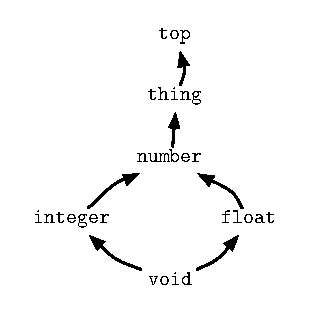
\includegraphics{number}}
\caption{\label{type:number}The type lattice associated with \q{number}}
\end{figure}

This lattice reflects the fact that integer and floating point values have separate internal representations.

A \q{number} is a \q{thing}
\begin{alltt}
number \impl thing.
\end{alltt}
which is how both \q{float}s and \q{integer}s are known to be \q{thing}s themselves.

\subsection{\q{logical} type}
\label{types:logical}
\index{type!logical@\q{logical}}
\index{logical@\q{logical} type}
The \q{logical} type is not primitive in the same sense that \q{char}, \q{number} and \q{symbol} are -- it can be defined using a \go algebraic type definition:
\begin{alltt}
logical ::= true | false.
\end{alltt}

\subsection{Tuple type}
\label{types:tuple}
\index{type!tuple}
\index{tuple!type of}
The tupling operator is the comma (\q{,}) operator. It is both a polymorphic type and a constructor for the tuple type. The tuple type is provided as a convenient way of grouping values together; but it has no interface per se. The tuple type is defined as though by:
\begin{alltt}
(,)[s,t] ::= (s,t)
\end{alltt}
where \q{s} and \q{t} represent the two degrees of polymorphic freedom available in a tuple. I.e., there is a single constructor for the tuple type: an infix \q{,} pair.

This, rather circular, definition highlights the fact that, in \go, the \q{,} infix operator is used both as the name of the tupling type as well as the tupling operator itself. It is, however, semantically, simply a predefined type with a single constructor that is very similar to a user-defined type.

The \q{,} operator is right associative, so it is possible to combine it into longer sequences:
\begin{alltt}
('joe',23,"his place",tonight)
\end{alltt}
is equivalent to:
\begin{alltt}
('joe',(23,("his place",tonight)))
\end{alltt}

\subsection{\q{list[]} type}
\label{types:list}
\index{type!list@\q{list}}
\index{list@\q{list[]} type}
The \q{list[]} type is the type used to denote sequences. The type interface for \q{list[]} is shown in Program~\ref{types:list:type}.
\begin{program}
\vspace{0.5ex}
\begin{alltt}
list[T] \impl{} \{
  head:[]=>T.
  tail:[]=>list[T].
  eof:[]\{\}.
  cons:[T]=>list[T].
  tack:[T]=>list[T].
  hdtl:[T,list[T]]\{\}
\}
\end{alltt}
\vspace{-2ex}
\caption{The \q{list[\_]} type interface}
\label{types:list:type}
\end{program}
This is one of the more complex standard types in \go with several elements in its interface:

\begin{description}
\item[\q{head}]
The \q{head} function method accesses the first element of the sequence. Note that although a \q{list[]} sequence can be implemented in a variety of ways, we require that the function method \q{head} (and the others in this interface) are \emph{pure} -- calling \q{head} of a \q{list[]} value will always return the same value.
\item[\q{tail}]
The \q{tail} function method accesses the remainder of the sequence.
\item[\q{eof}]
The \q{eof} predicate method is satisfied if the sequence is empty. Note that if the sequence is empty, then \q{head} and \q{tail} will raise an exception.
\item[\q{cons}]
The \q{cons} function returns a new stream with an element added to the \emph{beginning} of the sequence.
\item[\q{tack}]
The \q{tack} function returns a new stream with the element added to the \emph{end} of the sequence.
\item[\q{hdtl}]
The \q{hdtl} predicate is a convenience method -- it combines the \q{head} and \q{tail} operators into a single call. \q{hdtl} is used by \go in grammar rules: elements of a sequence that is parsed are accessed using the \q{hdtl} predicate method. For example, in the grammar rule:
\begin{alltt}
first:[list[char]]-->list[char].
first([X,..Y]) --> [X],\{letter(X)\},rest(Y).
\end{alltt}
the grammar terminal \q{[X]} is extracted from the stream using \q{hdtl}:
\begin{alltt}
S\sub0.hdtl(X,S\sub1)
\end{alltt}
where \q{S\sub0} represents the sequence of elements to parse at the beginning of the grammar rule, and \q{S\sub1} represents the sequence after having read \q{X}. For interest, the complete translation of this grammar rule in terms of sequences is:
\begin{alltt}
first([X,..Y],S\sub0,S\sub2) :-
  S\sub0.hdtl(X,S\sub1),
  letter(X),
  rest(Y,S\sub1,S\sub2).
\end{alltt}
\end{description}

Within \go the major implementation of the \q{list[]} interface is the list notation -- including \q{string}s. Other implementations of the \q{list[]} interface are possible, including, perhaps, one that permits a file to processed in a list-like manner.

\subsection{Function types}
\label{types:function}
\index{type!function}
\index{function!type}
\index{operator!=>@\q{=>}}
The function type is used to express the type of a function. We write function types as a left-hand side argument tuple type going to a result type:
\begin{alltt}
[T\sub1,\ldots,T\subn]=>T\sub{r}
\end{alltt}
Note that functions, and other programs, are \emph{not} \q{thing}s. Furthermore, these program types are \emph{not} permitted to be \emph{arguments} of other types -- other than in an interface type. This restriction reflects the fact that \go is not a higher-order programming language -- it is \emph{object ordered} instead.

The default \emph{mode} for a function type argument is \emph{input} -- written as \q{+}. However, it is possible to override this by suffixing a non-default mode; for example, in the type declaration:
\begin{alltt}
funnyOut:[integer,integer-]=>integer
\end{alltt}
The \q{funnyOut} function has its second argument as an \emph{output} argument. In effect, \q{funnyOut} returns a result in two channels: as its return value and by instantiating its second argument.

\subsection{Class constructor types}
\label{types:class}
\index{type!class constructor}
\index{class!constructor type}
\index{operator!\@=@\conarrow}
The class constructor type is used to express the types of constructor terms and enumerated symbols. There are two class constructor types, one for constructing statefree logical terms and one for constructing objects.

\subsubsection{Statefree class constructor type}

A statefree class constructor type has the form:
\begin{alltt}
[T\sub1,\ldots,T\subn]\conarrow{}T\sub{r}
\end{alltt}
An \emph{enumerated} symbol's type is distinguished from a constructor term's type by virtue of the fact that the left hand side of this type is empty:
\begin{alltt}
[]\conarrow{}T\sub{r}
\end{alltt}

All arguments of statefree constructor functions are, by definition, bi-directional. This cannot be overridden by attaching a mode declaration to the type; reflecting the fact that constructor functions are often used as \emph{patterns} as well as for naming results.

\subsubsection{Stateful class constructor type}
A stateful class constructor type has the form:
\begin{alltt}
[T\sub1,\ldots,T\subn]\sconarrow{}T\sub{r}
\end{alltt}
Note that, unlike statefree class constructors, there is no equivalent of the enumerated symbol for stateful classes. All stateful class constructors have arguments, although the arguments may be empty.

The arguments of a stateful class constructor are \emph{input}; reflecting the fact that stateful class constructors cannot be used as normal patterns. This permits the actual arguments of a stateful class constructor to a strict subtype of the requested type.

\subsection{Predicate types}
\label{types:predicate}
\index{type!predicate}
\index{predicate type}
The predicate type is used to express the type of a predicate. We write predicate types as a left-hand side argument tuple type followed by empty braces:
\begin{alltt}
[T\sub1,\ldots,T\subn]\{\}
\end{alltt}

The default mode for predicate type arguments is \emph{bi-directional} -- written as \q{-+}. This has two consequences: relational arguments are unified against and can pass information in two directions; and that the arguments to a relation may not be strictly lower than the type declared.

For example, if a relation is defined to be over \q{person}s:
\begin{alltt}
married:[person,person]\{\}
\end{alltt}
then any arguments in \emph{calls} to \q{married} must exactly of type \q{person}.

However, if we attached an \emph{input} mode to \q{married}'s first argument:
\begin{alltt}
married:[person+,person]\{\}
\end{alltt}
then the \q{married} relation definition will be compiled to \emph{expect} an actual value in the first argument -- just as for functions. 

In addition to this different semantics, marking the first argument of \q{married} as input also permits the type inference system to allow the first argument's type to be a sub-type of \q{person} -- a \q{student} perhaps.

\subsection{Action types}
\label{types:action}
\index{type!action}
\index{action!type}
The action type is used to express the type of a action procedure. We write action types as a left-hand side argument tuple type followed by an asterisk:
\begin{alltt}
[T\sub1,\ldots,T\subn]*
\end{alltt}

The default mode for action procedures is, like functions, input. However, it may be convenient and necessary for an action procedure to mark one or more of its arguments as \emph{output}:
\begin{alltt}
connect:[string,inChannel-]*
\end{alltt}
An output argument must be unbound at the time of the call to the action procedure; and it is normally expected (but not required) that the action procedure will instantiate that argument. In the case of \q{connect}, it is likely that the returned value will be one that can be used by a subsequent action.

\subsection{Grammar types}
\label{types:grammar}
\index{type!grammar}
\index{logic grammars!type}
\index{operator!-->@\q{-->}}
The grammar type is used to express the type of a grammar. We write grammar types as a left-hand side argument tuple type going to a sequence type:
\begin{alltt}
[T\sub1,\ldots,T\subn]-->list[T\sub{r}]
\end{alltt}
The sequence type should be a \q{list[]} type, as the grammar notation assumes that grammars are used to parse sequences.

Like predicates, the default mode for grammars is \emph{bi-directional}. Again, like predicates, this can be overridden selectively by marking the argument type. Grammar arguments tend to fall into one of two categories: constraints and parse tree outputs. The former is used to guide the parsing process -- such as:
\begin{alltt}
lookFor:[char] --> string.
lookFor(C) --> [C].
lookFor(C) --> [_], lookFor(C).
\end{alltt}
Such a constraint is often best catered for by marking the argument with an input mode suffix:
\begin{alltt}
lookFor:[char+] --> string.
\end{alltt}
Conversely, when building a parse tree as a side-effect of parsing a stream, the argument is often intended to be output only; in which case an output mode suffix would be indicated:
\begin{alltt}
factor:[parseTree-]-->string.
\end{alltt}

\section{Dealing with syntax errors}
\label{types:errors}
\index{type!dealing with errors}
Much as we would like to pretend otherwise, the main reason that we have a type system at all is to support the programmer in avoiding and correcting errors. In this section we look at some of the more common type problems and suggest strategies for dealing with them.

\subsection{The phases and kinds of error}
The order in which errors are reported by the compiler is not random -- it proceeds in distinct phases. If the compilation fails in an early phase then the later phases are not even attempted. This can lead to the potentially disheartening situation of apparently correcting the errors that are reported, only to uncover a whole set of new errors.

The phases that errors are reported in reflects the different phases of compilation itself:
\index{error!parse error}
\begin{description}
\item[parse errors] are reported over problems such as missing periods at the ends of rules, missing or extra parentheses and so on. Such errors are parse errors because they refer to the most surface-level aspects of the syntax of \go.

For example, if there is an extra period, as in:
\begin{alltt}
er\{
  tpe \impl{} \{p:[number]\{\}\}.

  lbl:[]\conarrow{}tpe.
  lbl..\{
    p(A) :- Q(A,B).
    .
    p(A).
  \}
\}
\end{alltt}
will be treated as a parse error; but may be confusing:
\index{error!close brace expected}
\begin{alltt}
Line er.go:5-8:
Syntax error: close brace expected,\ensuremath{\hookleftarrow{}}
     left brace at line: 5
Line er.go:1-6:
Syntax error: close brace expected,\ensuremath{\hookleftarrow{}}
     near p left brace at line 1
Line er.go:8:
Syntax error: TERM not permitted here
Line er.go:9:
Syntax error: \} not permitted here
Line er.go:10:
Syntax error: \} not permitted here
\end{alltt}
Most of the errors reported here are consequential -- caused by the first error but reported as the parser attempts to recover from the error.

The error message generated by the compiler is
\begin{alltt}
Line er.go:5-8:
Syntax error: close brace expected \ldots
\end{alltt}
not
\begin{alltt}
Line er.go:5-8:
Syntax error: extra period \ldots
\end{alltt}
because of the way that the compiler parses text. The presence of a period in the source -- particularly the terminator token which consists of a dot-space combination -- signals the end of an expression.

At the point where the parser sees the extra terminator it is not necessarily certain that this represents an error -- it needn't be.

\begin{aside}
As an example of where this kind of parsing behavior produces the correct result, consider the \q{*} operator. This is both an infix operator -- used in arithmetic expressions -- and a postfix operator -- used to mark the type of action procedures.

Thus the form:
\begin{alltt}
\emph{Exp} *.
\end{alltt}
is potentially legal -- at the parse level of the compiler -- and very similar to the text:
\begin{alltt}
\emph{Exp} . .
\end{alltt}
since \dotspace is also an infix and a postfix operator. Thus the potentially extra period cannot be reported as such because it may not be extra.

\go has a few operators that are both postfix and infix (or prefix): \q{;}, \q{*} and \q{\dotspace} itself.
\end{aside}
One unfortunate aspect of parse errors is that they do seem to generate a large number of consequential errors.

\index{error!ill-formed error}
\item[ill-formed errors]
The next phase after low-level parsing is the well-formed formedness test. This checks the shape of the input without considering type information or anything else to do with the semantics. The compiler also performs some source-level transformations at this stage.

It is this phase that reports errors about expressions being ill-formed, such as mixing up long predicate arrows (\q{:--}) with regular predicate arrows (\q{:-}).

Errors reported at this level often use the key phrase ``ill-formed" somewhere in the text. This can be taken as a hint as to the nature of the error found.

Due to the highly localized nature of well-formed formedness checking, locating and fixing such errors tends to be fairly straightforward. Note however, that the compiler only enters the next phase in the compilation process if no errors were detected in previous phases: only if there are no parse-level errors will you get any well-formed formedness errors.

\index{error!type error}
\item[type errors]
Type analysis is only performed on well formed programs. At this level the compiler attempts to ensure that arguments are applied to functions correctly and that it can compute the type of functions properly.

This is normally where most errors are reported; as the type checking stage represents the first significant semantic check on the program. Furthermore, some of the hardest to track errors are type errors.

\index{error!definition error}
\item[definition errors]
After successfully determining the types of identifiers, the compiler starts the compilation process -- itself in several phases. A definition error -- i.e., of a call to a program does not exist -- is raised at this level.

Also potentially raised at this level are errors such as attempting to assign to a variable that is not in scope, missing \q{valis} actions and so on.

\item[code generation errors]
are raised in the later stages of the compilation process. For example, if there is more than one occurrence of a variable in a matching context -- as in the left hand side of an equation -- then this will result in an error in the code generation phase.

On the whole, it is rare for code generation errors to be reported as hopefully the earlier stages of the process catches nearly all errors.
\end{description}

\index{error!invalid arguments}
\subsection{Invalid arguments to a program}
A most common kind of type error is likely to be incorrect arguments to a program of some kind.

The compiler automatically sorts the input program in order to ensure that whatever order the rules of the program are written in, type analysis always proceeds from the known to the unknown -- from the known types of programs to computing the type of the `current' program. This is one reason why the order of error reporting often does not at all reflect the text order in the program source.

When a type error occurs as a result of an invalid type of argument, the compiler will try to highlight the problem -- in addition to marking the error it will try to point out the particular aspect of the incorrect types.

Note that if the \emph{arity} of a call to a program is wrong, then only the fact that the arity is wrong will be reported. The compiler does not attempt to go into the arguments to see which argument may be missing or extra.



%\subsection{Issues with declaring types and interfaces}
%\label{type:occur}

%\index{error!in type declaration}
%Suppose that we wished to define an interface that encapsulated what it meant to be comparable. A first definition of this interface might look like \q{comp[]} in Program~\vref{type:comp:1}.
%\begin{program}
%\vspace{0.5ex}
%\begin{verbatim}
%comp[T] <~ { equal:(T){} }.
%\end{verbatim}
%\vspace{-2ex}
%\caption{A first \q{comp}arable type interface}
%\label{type:comp:1}
%\end{program}
%While this type definition is technically fine, it does have a usability issue.  A na\"ive first attempt at a class that implements the \q{comp[]} type might be:
%\begin{alltt}
%cmp:comp[_]..\{
%  equal(this).
%\}
%\end{alltt}
%However, trying to compile this program would result in an occurs check type error:
%\begin{alltt}
%Syntax error: type of equal:(comp[\_t10])\{\}
%  not consistent with required type: (\_t10)\{\}
%because occurs check: \_t10 in comp[\_t10]
%\end{alltt}
%\index{occurs check}
%An occurs check is signaled when trying to unify a variable against a term ( type term or otherwise) that contains the variable being unified against. If permitted, such a unification sets up a cycle that implies  that the type term is actually infinite in size -- which is not permitted in standard interpretations of first order logic.

%The initial reason for this error is that the type interface for \q{comp} in example~\vref{type:comp:1} requires that the argument to the \q{equal} predicate method is a \q{T}, not an \q{comp[T]} value.

%What we \emph{should} have done is define the \q{comp[]} type so that its \q{equal} predicate took a \q{comp[T]} as an argument, instead of just \q{T}; as in Program~\vref{type:comp:2}. With this definition, our \q{cmp} class above compiles without errors.
%\begin{program}
%\vspace{0.5ex}
%\begin{verbatim}
%comp[T] <~ { equal:(comp[T]){} }
%\end{verbatim}
%\vspace{-2ex}
%\caption{\label{type:comp:2}A recursive \q{comp[]} interface}
%\end{program}
%However, this program suffers from a different problem: the \q{equal} predicate method requires a \q{comp[T]} argument, which effectively restricts the utility of the type -- as the only thing published by \q{comp[]} is the \q{equal} predicate, that is the only use that a \q{comp[]} entity can be put to.

%A more useful form would be where the \q{equal} predicate took any argument that \emph{implements} the \q{comp[T]} interface. We can see an attempt to do this in program~\vref{type:comp:3}.
%\begin{program}
%\vspace{0.5ex}
%\begin{verbatim}
%comp[T] <~ { equal:(T<~comp[T]){} }.

%other[T] <~ comp[T].
%other[T] <~ { more:(()=>T) }.

%d(X):other[T]..{
%  equal(this).

%  more()=>X
%}
%\end{verbatim}
%\vspace{-2ex}
%\caption{\label{type:comp:3}An implements-style \q{comp[]} interface}
%\end{program}
%This program however itself raises a syntax error. The error raised is an occurs check in the definition of \q{equal} within the \q{d()} class.

%It turns out that there is no way of implementing the \q{comp[]} interface as shown in program~\vref{type:comp:3}. Any attempt will raise an occurs check.

%The deep reason for this is that the way that \q{comp[]} is written -- where the \q{equal} predicate takes the same type as that of the class implementing \q{comp[]} -- is flawed and against the spirit of the implements type relationship.

%We use the type implements relationship -- in contrast to the type equality relationship -- when we want to permit any argument that implements the interface in a function (say). However, that requirement is in conflict with the implicit assumption in a polymorphic type that the types are identical.

%The \emph{appropriate} way of defining a usable \q{comp} type is shown in program~\vref{type:comp:4}. In that definition, \q{comp} is not polymorphic, although the \q{equal\{\}} predicate method defined within it is.
%\begin{program}
%\vspace{0.5ex}
%\begin{verbatim}
%comp <~ { equal:[T]-[T<~comp]{} }.

%other[_] <~ comp.
%other[T] <~ { more:[]=>other[T] }.

%d(X):other[T]..{
%  equal(this).
%  
%  more()=>this.
%}
%\end{verbatim}
%\vspace{-2ex}
%\caption{\label{type:comp:4}A non-polymorphic \q{comp} type}
%\end{program}

%The lesson here, it seems, is that when defining a type that is intended to be inherited -- as in the case of \q{comp} -- then it should be defined to be non-polymorphic. It is, in principle, possible to have a type that is polymorphic and inheritable, but either such type is not recursive or it will not be all that useful -- because to avoid occurs check-type errors ...

\subsection{Singleton variables}
\label{type:singleton}
\index{variable!singleton occurrence}
Although not technically an error, the compiler will warn when it finds only one occurrence of a variable. The reason is that such occurrences are often errors in disguise: a typo can cause an apparently well formed identifier to be misunderstood.

The compiler does \emph{not} issue a warning, however, if the variable's identifier's first character is an underscore. This allows you to explicitly mark singleton occurrences -- they are singleton and you know it.

The \go compiler has very few warnings in its repertoire -- either a particular syntactic construction is perfectly valid or its not. The compiler will warn you when you apparently try to redefine a built-in escape and also it tries to enforce the regimen that type names are suffixed with \q{[]}.

\subsection{Implicit exporting of private types}
\label{type:implicit:export}
\index{export!implicit  export of type}
A package's definitions are normally exported unless they are marked \emph{private}. Any definition can be marked private, including types -- after all there may be occasions where a type is intended to be used internally only.

However, if a \emph{type} is marked \q{private}, then some care must be taken. If an exported program references a private type then, potentially, that type is effectively exported. At the least, any package that imported such a program would have problems dealing with the implicitly exported type -- the best you can hope for is that it becomes a kind of opaque type.

Since it is potentially an error, the compiler will generate a warning if a private type is referenced by any element that is exported.







